\documentclass[a4paper,12pt,fleqn]{article}
\usepackage[T1]{fontenc}
\usepackage{ucs}
\usepackage[utf8x]{inputenc}
\usepackage{ngerman}
\usepackage[ngerman]{babel}
\usepackage{lastpage}
\usepackage[pdftex]{color,graphicx}
\usepackage{listings}
\usepackage{pdflscape}
\usepackage{longtable}
\usepackage[inner=2cm,outer=2cm,top=1cm,bottom=1.5cm,includeheadfoot]{geometry}
\usepackage{fancyhdr}
\usepackage{url}
\usepackage{pgfgantt}
\usepackage{amsmath,amssymb,amsfonts,amstext}

% highlighting
\usepackage{xcolor,soul}

%---- PageLayout
\pagestyle{fancy}

\setlength{\headsep}{10mm}

\usepackage{eso-pic}

%----------------------------------------------------------------------------
% HEADER --------------------------------------------------------------------
%----------------------------------------------------------------------------
\fancyhead[R]{
  
\includegraphics[width=100pt,keepaspectratio]{img/amedo2012.png}
}

\fancyhead[C]{ Pflichtenheft }

\fancyhead[L]{
  \begin{tabular}[b]{l}
  Christoph Gnip\\
  Projekt: PRPS-Evo
  \end{tabular}
}

%Linie oben
\renewcommand{\headrulewidth}{0.5pt}
%---------------------------------------------------------------------------
\fancyfoot[L]{Stand: \today}
\fancyfoot[C]{ }
\fancyfoot[R]{\thepage{} von \pageref{LastPage}}

% Linie unten
\renewcommand{\footrulewidth}{0.5pt}
%----------------------------------------------------------------------------

% Import Macros  ------------------------------------------------------------
%\newcommand\nn{\newline\newline}

%----------------------------------------------------------------------------
% Start the Document --------------------------------------------------------
%----------------------------------------------------------------------------
\begin{document}

%\definecolor{barblue}{RGB}{153,204,254}
%\definecolor{groupblue}{RGB}{51,102,254}
%\definecolor{linkred}{RGB}{165,0,33}
%\renewcommand\sfdefault{phv}
%\renewcommand\mddefault{mc}
%\renewcommand\bfdefault{bc}
%\sffamily

\setlength{\headheight}{36pt}

\begin{titlepage}


%- the Title page --------------------------------------------------------
\begin{center}
%\vspace*{2.5cm}
{\Huge \textbf{Pflichtenheft zur Master-Thesis}\par}
\vspace{1cm}

{\large Titel: \\
\textbf{Entwicklung eines Systems zur Entfernungsabschätzung für
Phasen basiertes UHF RFID Tracking durch Verwendung evolutionärer Berechnungsverfahren}\par}
\vspace{1cm}

{\large Projektname:\\ 
\textbf{PRPS-Evo}\par}

\vspace{2cm}

\large{Erstellt durch}\\
\Large{\textbf{Christoph Gnip}}

%\vspace{4cm}
\vfill

{\normalsize Fachbereich Elektrotechnik und angewandte Naturwissenschaften\\
Westfälische Hochschule\\[2ex]Mai 2013}


\end{center}
\newpage

\end{titlepage}

%----------------------------------------------------------------------------
\begin{abstract}
Dieses Dokument beschreibt ausführlich die Aufgabenstellung der Masterarbeit von Christoph M. Gnip. Es ist in Form eines Pflichtenheftes aufgebaut.
\end{abstract}

%----------------------------------------------------------------------------
%own page for the toc
\tableofcontents
\newpage

%----------------------------------------------------------------------------
\section{Motivation}
Die Positionsbestimmung (Tracking) mittels RFID (Radio-Frequency Identification) bietet gegenüber vergleichbaren Methoden (z.B. Ultraschall, Optisch) verschiedene Vorteile. Das wesentlichste Unterscheidungsmerkmal ist, dass keine direkte Sichtlinie sog. LOS (Line of Sight) notwendig ist um ein Objekt zu lokalisieren. Der Grund dafür ist das zugrunde liegende Messprinzip. Insbesondere im Vergleich mit optischen Verfahren ist RFID damit überlegen. Weiterhin erlauben die als Positionsgeber verwendeten Tags zusätzliche Informationen auf ihnen abzulegen, beispielsweise eine Identifikationsnummer und Weiteres. Dadurch wächst das Anwendungsspektrum weiter. Das Auslesen von zusätzlichen Informationen ist in keiner der anderen Technologien möglich.\\

Das von dem Messsystem der {Amedo GmbH} verwendete Verfahren basiert auf der Messung der Phasenlage der Antwort eines Tags. Die Phasenlage ist direkt proportional zu einer Entfernung. Dabei kommt es aufgrund der Physik im wesentlichen zu folgenden Problemen:
\begin{enumerate}
	\item Die Messung der Position erfolgt über die Auswertung der Phasenlage des empfangenen Signals in Bezug auf ein Referenzsignal. Da in der EU sind nur bestimmte Frequenzen für die Verwendung für RFID erlaubt (865,5–867,5 MHz) kann man die Wellenlänge mit: $ \lambda\simeq0,35 m $ angeben. Daraus folgt, dass alle 35 cm die gleiche Konfiguration der Phase vorliegt. In dieser Arbeit wird dieser Umstand Isophasen genannt. Die gewonnene Information aus der Phase ist somit redundant, d.h. es lässt sich durch die Kenntnis der Phase nicht unmittelbar auf die korrekte Postion schließen. Man kann das Problem umgehen in dem man auf die errechnete Position ein ganzzahliges Vielfaches der Wellenlänge addiert. Die sog. Wellenzahl (vgl.~\eqref{eq:Wavenumbers}).
	\item Das System der Amedo STS verwendet eine spezielle Antennenanordnung um die Position zu ermitteln. Dabei wird eine Antennenanzahl >4 eingesetzt. Für jede dieser Antennen muss eine eigene Wellenzahl bestimmt werden. Durch Auslöschung des Signals, Absorption etc. kann es dazu kommen, dass eine Antenne eine unbestimmte Zeit lang kein Signal vom Tag empfängt. Wenn die Antenne nach dieser Zeit erneut ein Signal empfängt ist die ihr zugehörige Wellenzahl unbekannt und muss neu bestimmt werden. 
	\item In realen Umgebungen treten zusätzlich noch Ruflektionen und ein sog. Multipath-Effekt auf. Dabei wird das Signal nicht auf dem Direkten Weg Antenne-Tag-Antenne empfangen sondern über einen unbekannten, längeren Weg. Dadurch kommt es zu einem Fehler in der Phase. Zusätzlich ist dieser Effekt individuell für jede Antenne.
\end{enumerate}

Eine analytische Lösung des Problems ist schwierig und bisher nicht gelungen. In dieser Arbeit soll mittels numerischer Methoden und Modellen die beschriebenen Probleme zu gelöst werden.

%
%Das Problem liegt in den unbekannten, komplex zu modellierenden Verhalten der elektromagnetischen Funkwellen in geschlossenen Räumen (insb. Auslöschung, Multipath, Reflektion). Diese führen zu einem Fehler der Phase und damit direkt zu einer Falschaussage der Position.\\ \\
%\textbf{Beschreibung der Wellenzahl[Referenz auf die Dipl. Arbeit von Bernd]}\\\\
%Ziel dieser Arbeit ist es ein System zu
%implementieren, das eine direkte Abschätzung (Ad-Hoc-Messung) der Wellenzahl erlaubt.
%Dafür werden Methoden der Numerik verwendet um die Uneindeutigkeit der Phasenlage zu
%eliminieren.
%\\ \\ \\
%Tags gibt es mit unterschiedlichen Funktionsweisen, in dieser Arbeit und in dem von der {Amedo STS} verwendeten System kommen passive Tags zum Einsatz. Diese versorgen sich aus den Funksignalen des Abfragegeräts mit der notwendigen Energie und modulieren ihre "Antwort" auf das Trägersignal auf.\\\\\\
%In der Positionsbestimmung wird im Zusammenhang von "Marker" gesprochen. In der in dieser Arbeit werden RFID-Transponder (sog. Tags) als Marker verwendet. D.h. Es wird die Position im Raum von einem Transponder ermittelt. \\
%


%----------------------------------------------------------------------------
\section{Aufgabenstellung}
Im Folgenden ist die Aufgabenstellung detailliert ausgeführt. Die Anforderungen der Arbeit sind in Muss-, Soll- und Wunschkriterien unterteilt. Entsprechend dieser Einteilung ergibt sich die Priorität der Aufgaben.

\subsection{Musskriterien}
Ziel dieser Arbeit ist es ein System zu entwerfen und umzusetzen, das die eingangs beschriebene Problematik, der unbekannten, nicht analytisch bestimmbaren Wellenzahl löst. Dazu sollen evolutionäre Verfahren verwendet werden. Zu Beginn der Arbeit wird eine State of the Art-Erhebung durchgeführt, um die geeignetste Methode zu finden. In Vor

\subsection{Sollkriterien}
Die Vorarbeiten zu diesem Projekt lassen erwarten, dass die aktuell vorliegenden Messdaten nur bedingt für die Auswertung verwendet werden können. Sollte sich diese Annahme im Laufe der Arbeit bestätigen, sind entsprechende Maßnahmen zu treffen, denkbar wären:
\begin{itemize}
\item Filterung der Daten
\item Anpassung der Messdatenaufnahme
\end{itemize}

\subsection{Wunschkriterien}
Ein in der Bearbeitung impliziertes Problem betrifft die Kalibrierung des Systems. Es ist sehr erstrebenswert, dass die Ergebnisse dieser Arbeit auch einen Lösungsansatz zu dieser Problemstellung liefern. In Vorüberlegungen zu dieser Arbeit wurden Abschätzungen vorgenommen über die Realisierbarkeit der Aufgabe, dabei wurde auch ein Lösungsansatz mittels Neuronaler Netze diskutiert. Die Beurteilung dieses Ansatzes umfasst, dass es zur Zeit nicht praktikabel ist die entsprechend große Anzahl an Datensätzen zu generieren, der Ansatz generell vielversprechend ist. Es ist davon auszugehen, dass im Rahmen der Kalibrierung ausreichend viele Daten anfallen, um ein Neuronales Netz zu trainieren. Wenn es in die Bearbeitungszeit der Arbeit passt, wird dieser Ansatz weiter verfolgt.

\subsection{Abgrenzungskriterien}
Algorithmen und Testanordnungen welche bereits entwickelt wurden sind einzusetzen und nicht neu zu erfinden. Es dürfen/ sollen alle bereits erbrachten Arbeitsergebnisse der Amedo STS genutzt werden und werden in dieser Masterarbeit mit entsprechender Quellenangabe verwendet werden.

%----------------------------------------------------------------------------
\section{Umsetzung}
Dieses Kapitel beschreibt die beabsichtigte Herangehensweise des Autors an die
ihm gestellte Aufgabenstellung. Aus den Beschreibungen geht hervor welche Schritte durchgeführt werden um das Projekt zu bearbeiten.

\subsection{Problembeschreibung}

Die Entfernungsmessung über die Phasenlage des Empfangenen Signals kann durch folgende Gleichung beschrieben werden:

%\begin{equation}
\begin{alignat}{2}\label{eq:Wavenumbers}
 	d(\Theta)&=\frac{\lambda}{2}(\frac{\Theta}{2\pi}+n) &\quad
 	,\lambda&=\frac{c}{\nu}
\end{alignat}

$d(\Theta)$ meint die Distanz von einem Tag für eine bekannte Phase $\Theta$
       
% \qquad \text{Maxwell's equations}
%\end{equation}



%----------------------------------------------------------------------------
\section{Systemkenndaten}
%----------------------------------------------------------------------------
\subsection{Hardware}
Das Projekt verwendet das PRPS-System der Amedo STS. Es handelt sich dabei um ein System aus mehreren Antennen, die mehrere RFID-Tags ausmessen können. Die Messdatenaufnahme erfolgt durch einen leistungsstarken FPGA (Field Programmable Gate Array). In dem System steht ein PC mit dem Betriebssystem Ubuntu zur Verfügung. Nach der Vorverarbeitung durch den FPGA werden die Daten zu dem PC übertragen und dort die abschließende Positionsberechnung durchgeführt. Die Schnittstelle zum Endkunden/ andere Software erfolgt via TCP/IP und dem PRPS-Protokoll. Über das Protokoll kann die Hardware gesteuert werden.\\
Weiterhin steht ein CNC-gesteuerter Lineartisch für die Messdatenaufnahme zur Verfügung.


%----------------------------------------------------------------------------
\subsection{Software}
Für die Steuerung der Hardware wird das Tool AmedoPRPSHow eingesetzt. Dabei handelt es sich um eine der Entwicklung dienende Software, die es ermöglicht über das PRPS-Protokoll das PRPS-System zu steuern, die Daten zu empfangen und zu visualisieren.\\
In den Vorgesprächen zu dieser Arbeit wurde die Softwareplattform: Shark entdeckt. Shark ist eine Library, die bereits viele evolutionäre Methoden beinhaltet. Im Rahmen dieser Arbeit soll sie verwendet werden, da sie die Referenzimplementierung für dem CMA-ES-Algorithmus ist. Weiterhin ist sie in C++ geschrieben und ermöglicht so eine einfache Portierung auf andere Plattformen.\\
Im Rahmen dieser Arbeit steht Matlab in der Version 2013b zur Verfügung. Der Einsatz von Matlab kann bei vielen Teilen der Arbeit als nützlich sein. Besonders bei einem voraussichtlichem Filterentwurf.  


%----------------------------------------------------------------------------
\subsection{Werkzeuge und Umgebungen}
\subsubsection{Quellcodeverwaltung}
In dieser Arbeit wird das Quelloffene Versionsverwaltungssystem Git verwendet.
Das Repository wird auf den Servern des Web-dienst ''GitHub.com'' hinterlegt um
einen Austausch zwischen den verschiedenen Umgebungen zu erleichtern. Dieses
Repository stellt eine weitere Ausfallsicherheit dar, das Risiko eines
Datenverlustes wird so erheblich reduziert. Gleichzeitig wird großen Wert auf
die Sicherheit und Integrität der Daten gelegt. Wie im Folgenden
genauer beschreiben.

%----------------------------------------------------------------------------
\subsubsection{Programmierung}
Die Software, die in diesem Projekt erstellt wird, muss auf dem Linux-Rechner im PRPS lauffähig sein. Die Entwicklungsumgebung sollte aus Gründen der Einfachheit daher entweder die Möglichkeit zur Cross-Kompilierung bieten oder eine direkte Portierung der erstellten Programme ermöglichen. Am geeignetsten für diese Aufgabe stellt sich die IDE (Integrated Development Environment) Eclipse heraus. Es wird die Herlios Version verwendet. Die Wahl des Betriebssystems fällt auf Ubuntu 12.04 LTS für die Programmierumgebung. Dabei wird die Umgebung in einer Virtuellen Maschine unter der Verwendung von Oracle Virtual Box aufgesetzt. Dies ermöglicht eine einfache Portierung und Dokumentation, da die Gesamte Maschine einfach zwischen verschiedenen Rechnen und Betriebssystemen kopiert werden kann.

%----------------------------------------------------------------------------
\subsubsection{Dokumentation}
Die Projektdokumentation wird in \LaTeX{} erstellt. Eine entsprechende Umgebung ist auf allen in dem Projekt verwendeten Rechner aufzusetzen.\\
Während des Projekts wird in auf wöchentlicher Basis ein Bericht angefertigt aus dem der aktuelle Projektstand hervorgeht.

%----------------------------------------------------------------------------
\section{Projektplanung}
Die Dauer der Arbeit beträgt 20 Wochen. Start in der KW 17. Abgabe des Projekts ist am 9. September 2013.
\subsection{Projektlaufplan}
Siehe~\ref{sec:projectplan}

%----------------------------------------------------------------------------
%- Appendix ------------------------------------------------------------------
%
%
%
\begin{appendix}

%----------------------------------------------------------------------------
%----------------------------------------------------------------------------
%\newpage
%
%\begin{center}
%	\huge{Anhänge}
%\end{center}

\normalsize
%
%----------------------------------------------------------------------------
%----------------------------------------------------------------------------
\chapter{Abbildungen}
\section{Messaufbauten}
\begin{figure}[h!]
 \centering
         \includegraphics[width=\textwidth]{img/00_Placeholder.png}
         \caption[PRPS-Kalibiersystem]{PRPS-Messsystem in der "Spinnen"-Konfiguration. Es umfasst vier Messwertgeber und eine Recheneinheit.}
         \label{fig:Spider1}
\end{figure}
\newpage
%
%----------------------------------------------------------------------------
%----------------------------------------------------------------------------
\begin{figure}[h!]
 \centering
         \includegraphics[width=\textwidth]{img/00_Placeholder.png}
         \caption[Übersicht Kalibrieraufbau]{Aufbau des für die Kalibrierung verwendeten Messaufbaus.}
         \label{fig:Spider_setup1}
\end{figure}
\newpage
%
%----------------------------------------------------------------------------
%----------------------------------------------------------------------------
\chapter{Gnuplot Skripte}
\section{Boxplot}
\tiny
\lstinputlisting[
		title=Gnuplot Boxplot-Skript,
		caption=Gnuplot Boxplot-Skript,
		language=Gnuplot,
		numbers=left,
%		frameround=fttt,
		frame=trbl,
		breakatwhitespace=false,         % sets if automatic breaks should only happen at whitespace
   	    breaklines=true,  
		xleftmargin=1cm,
		showstringspaces=false]{../../dev/src/c-cpp/AntConfApp/build/Debug/test/output/mkII/plot/kondensierte_boxen.gp}
\label{append_Script_Box-plot}
\newpage
%
%----------------------------------------------------------------------------
%----------------------------------------------------------------------------
\section{Lineplot}
%\begin{footnote}
\tiny 
%
% listings print source code

% define colors for source code list
\definecolor{colKeys}{rgb}{0,0,1}
\definecolor{colIdentifier}{rgb}{0,0,0}
\definecolor{colComments}{rgb}{0,1,0.3}
\definecolor{colString}{rgb}{0,0.5,0}

\definecolor{dkgreen}{rgb}{0,0.6,0}
\definecolor{gray}{rgb}{0.5,0.5,0.5}

\lstset{language=Matlab,
   keywords={break,case,catch,continue,else,elseif,end,for,function,
   global,if,otherwise,persistent,return,switch,try,while,ones,zeros},
   float=hbp,
   basicstyle=\ttfamily\small,
   identifierstyle=\color{colIdentifier},
   keywordstyle=\color{blue},
   commentstyle=\color{dkgreen},
   stringstyle=\color{red},
   columns=flexible,
   tabsize=2,
   frame=single,
   numbers=left,
   extendedchars=true,
   showspaces=false,
   numberstyle=\tiny\color{gray},
   stepnumber=1,
   numbersep=10pt,
   showspaces=false,
   showstringspaces=false,
   breakautoindent=true}

\lstinputlisting[
		title=Gnuplot Lineplot-Skript,
		caption=Gnuplot Lineplot-Skript,
		language=Gnuplot,
		numbers=left,
%		frameround=fttt,
		frame=trbl,
		breakatwhitespace=false,         % sets if automatic breaks should only happen at whitespace
   	    breaklines=true,  
		xleftmargin=1cm,
		showstringspaces=false]{../../dev/src/c-cpp/AntConfApp/build/Debug/test/output/mkII/plot/kondensierte_linien.gp}
\label{append_Script_Line-plot}
\newpage
%
%----------------------------------------------------------------------------
%----------------------------------------------------------------------------
\section{Scatterplot}
%\begin{footnote}
%
% listings print source code

% define colors for source code list
\definecolor{colKeys}{rgb}{0,0,1}
\definecolor{colIdentifier}{rgb}{0,0,0}
\definecolor{colComments}{rgb}{0,1,0.3}
\definecolor{colString}{rgb}{0,0.5,0}

\definecolor{dkgreen}{rgb}{0,0.6,0}
\definecolor{gray}{rgb}{0.5,0.5,0.5}

\lstset{language=Matlab,
   keywords={break,case,catch,continue,else,elseif,end,for,function,
   global,if,otherwise,persistent,return,switch,try,while,ones,zeros},
   float=hbp,
   basicstyle=\ttfamily\small,
   identifierstyle=\color{colIdentifier},
   keywordstyle=\color{blue},
   commentstyle=\color{dkgreen},
   stringstyle=\color{red},
   columns=flexible,
   tabsize=2,
   frame=single,
   numbers=left,
   extendedchars=true,
   showspaces=false,
   numberstyle=\tiny\color{gray},
   stepnumber=1,
   numbersep=10pt,
   showspaces=false,
   showstringspaces=false,
   breakautoindent=true}

\tiny
\lstinputlisting[
		title=Gnuplot Scatterplot-Skript,
		caption=Gnuplot Scatterplot-Skript,
		language=Gnuplot,
		numbers=left,
%		frameround=fttt,
		frame=trbl,
		breakatwhitespace=false,         % sets if automatic breaks should only happen at whitespace
   	    breaklines=true,  
		xleftmargin=1cm,
		showstringspaces=false]{../../dev/src/c-cpp/AntConfApp/build/Debug/test/output/mkII/plot/scatter.gp}
\label{append_Script_Scatter-plot}
\newpage
%
%----------------------------------------------------------------------------
%----------------------------------------------------------------------------
%\section{Filter Entwurf - Ergebnisse}
%\begin{landscape}
%\label{FirFilterResult}
%\begin{figure} [h]
         \centering
         \caption{ Ergebnisse des Filterentwurfs }
         \label{fig:1}
         \centering
         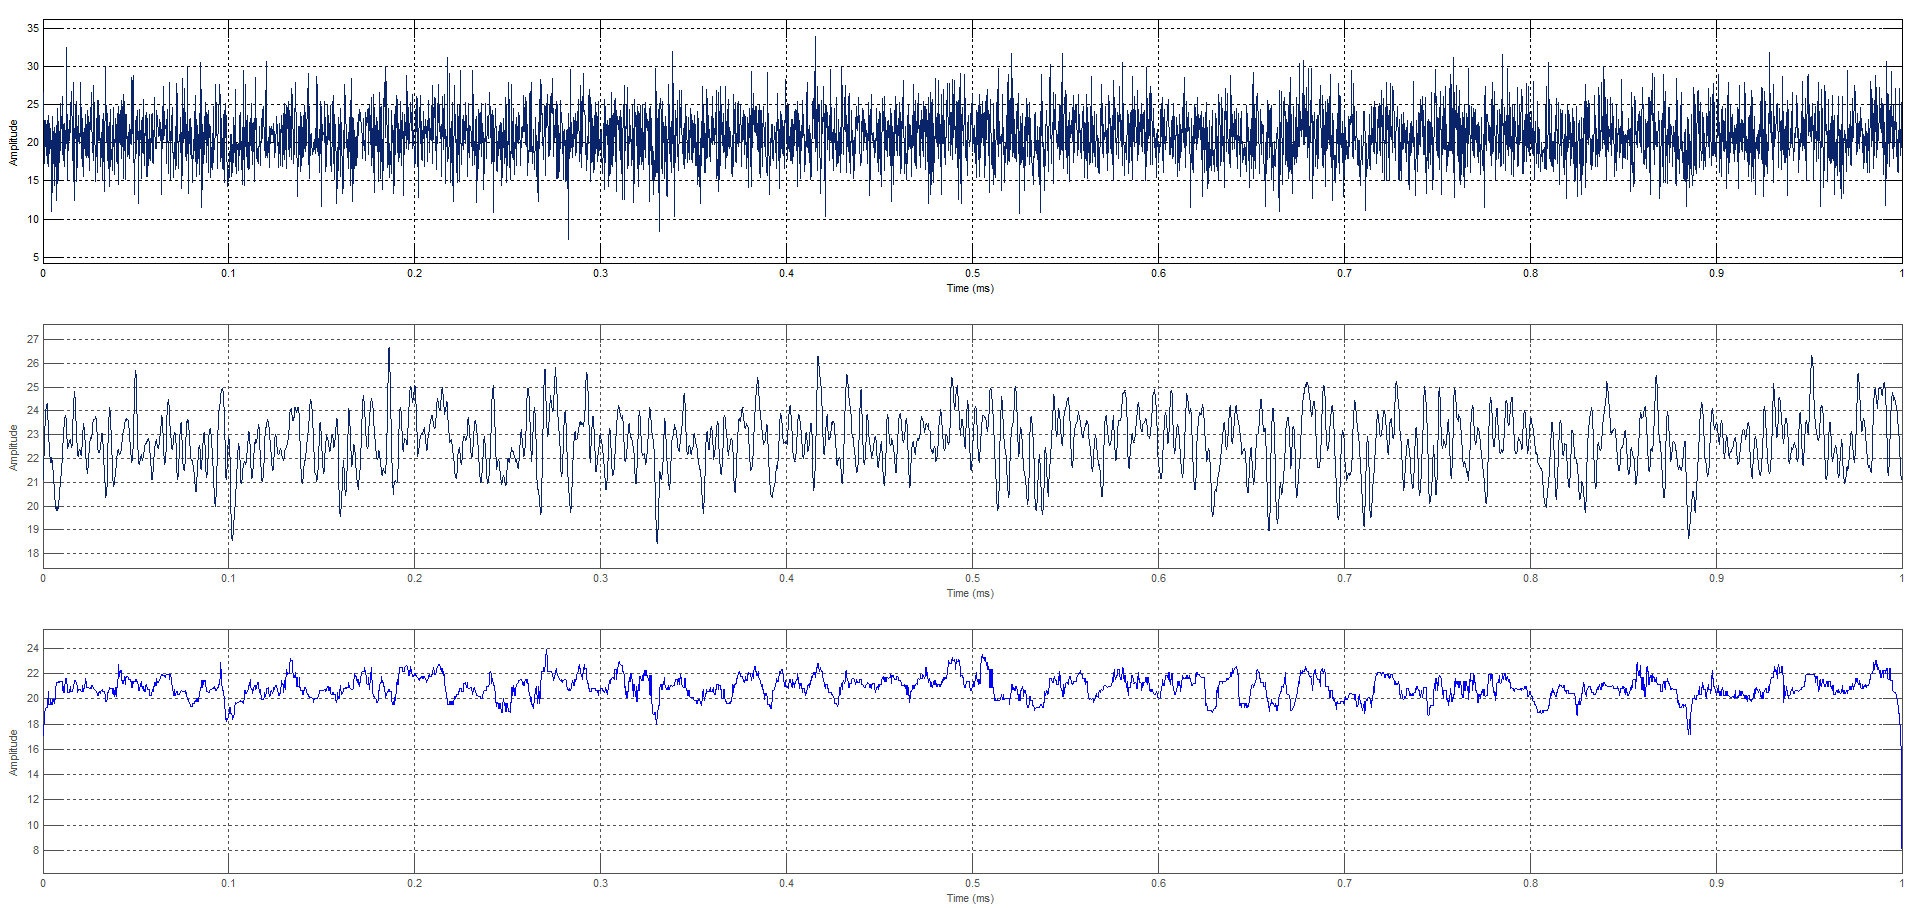
\includegraphics[width=.8\textwidth]{common/img/AmpGefiltert_small.png}\\
\vspace{0.5cm}
Die obere Kurve visualisiert die Rohdaten. Die mittlere Kurve ist das Ergebnis der Tiefpassfilterung für einen der vorgestellten Filter. Die untere Darstellung dient zum Vergleich mit der bisher eingesetzten Filterungsmethode (Median). Es wurden 4096 Messwerte für diese Analyse gesampelt.
\end{figure}
%---------------------------------------------------------------------------------------
\vspace{.5cm}
%---------------------------------------------------------------------------------------
\begin{figure} [h]
         \centering
         \caption{ Spektrum des Messsignals, vor und nach der Filterung  }
         \label{fig:2}
	     \centering
	     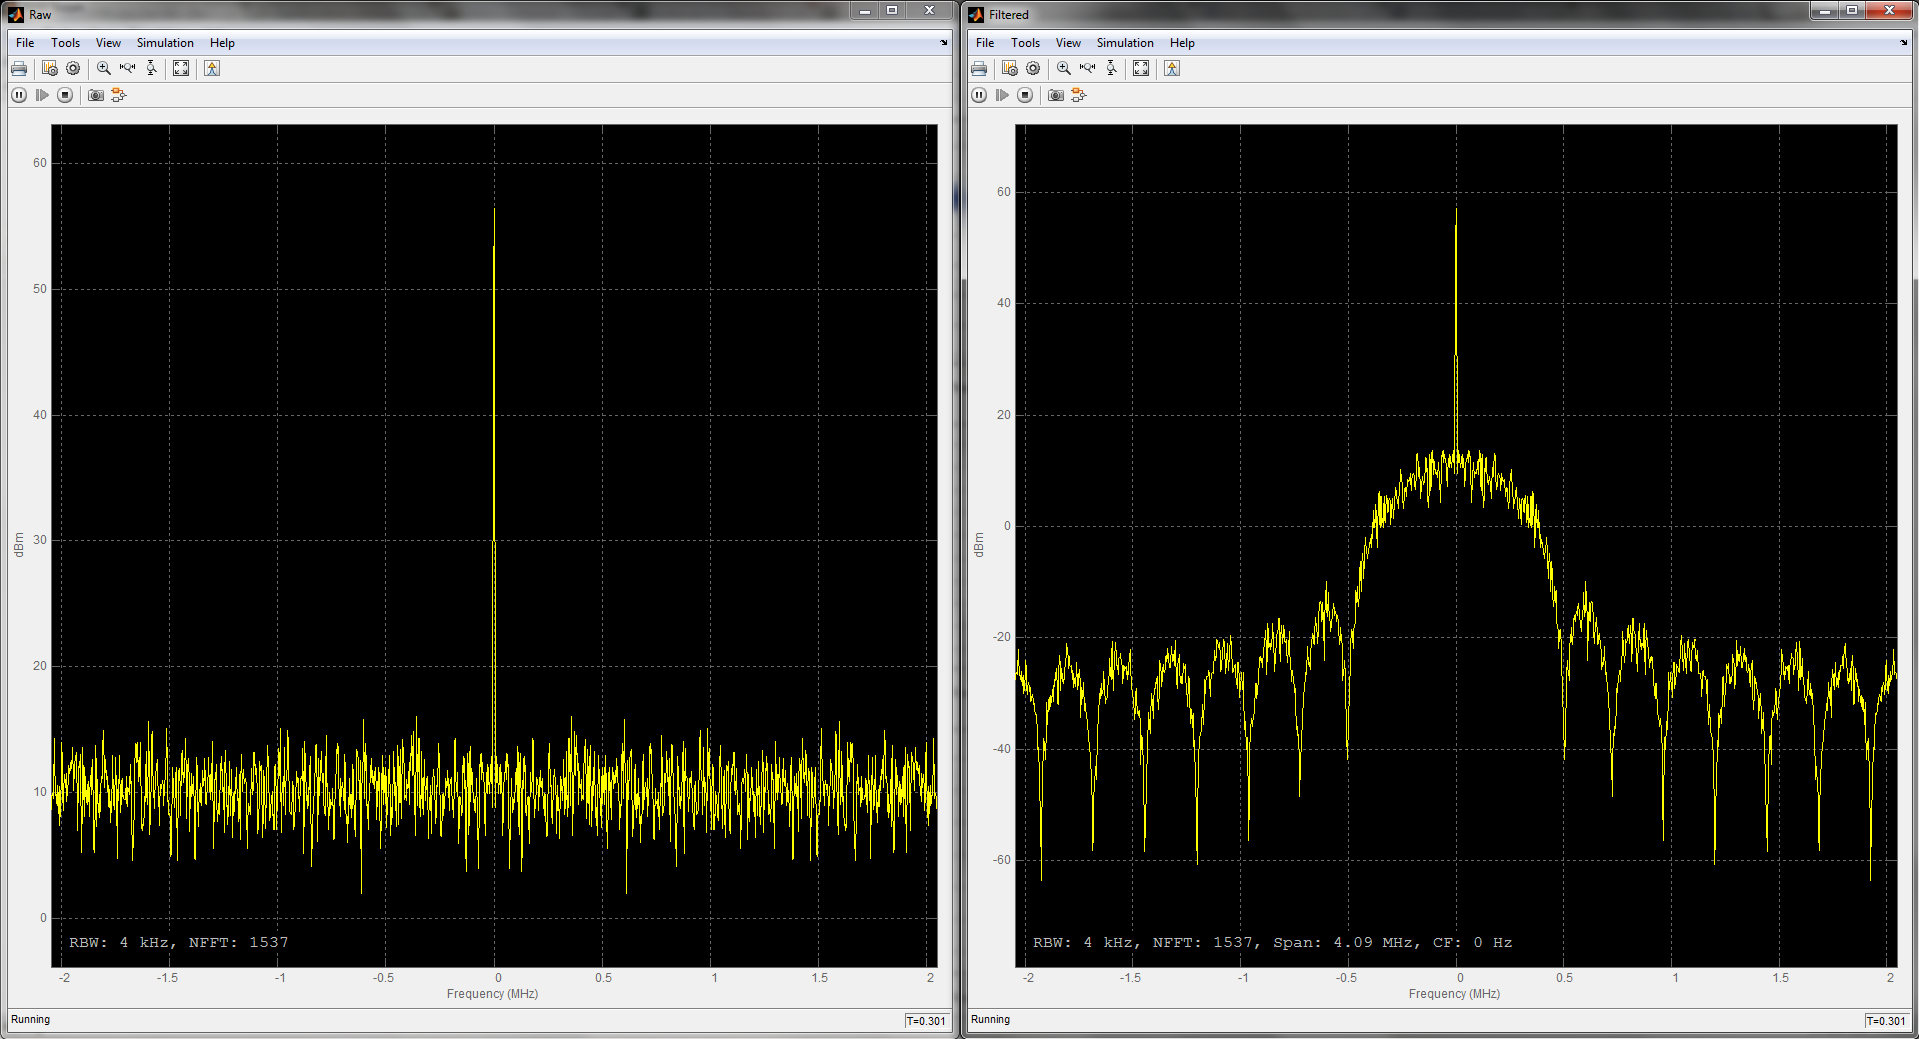
\includegraphics[width=.6\textwidth]{common/img/SpektrumAmp.PNG} \\
\vspace{.2cm}
Die Grafik zeigt das Spektrum des Messsignals der Amplitude. Im linken Bild ist das ungefilterte Signal und im Rechten das gefilterte.
%
\end{figure}
%---------------------------------------------------------------------------------------
\vspace{.5cm}
%---------------------------------------------------------------------------------------
\begin{figure} [h]
         \centering
         \caption{ Frequenzgänge der entworfenen Filter. Beide ähneln sich in den Parametern, verfügen jedoch über etwas unterschiedliche Eckfrequenzen. Als Entwurfsmethode wurde die sog. "Least-squares"-Methode verwendet. Diese Methode liefert gute Ergebnisse im Hinblick auf möglichst kleine Sidelobes und eine geringe Anzahl an Koeffizienten. }
         \label{fig:3}
%         
         \begin{subfigure}[t]{0.5\textwidth}
                 \centering
                 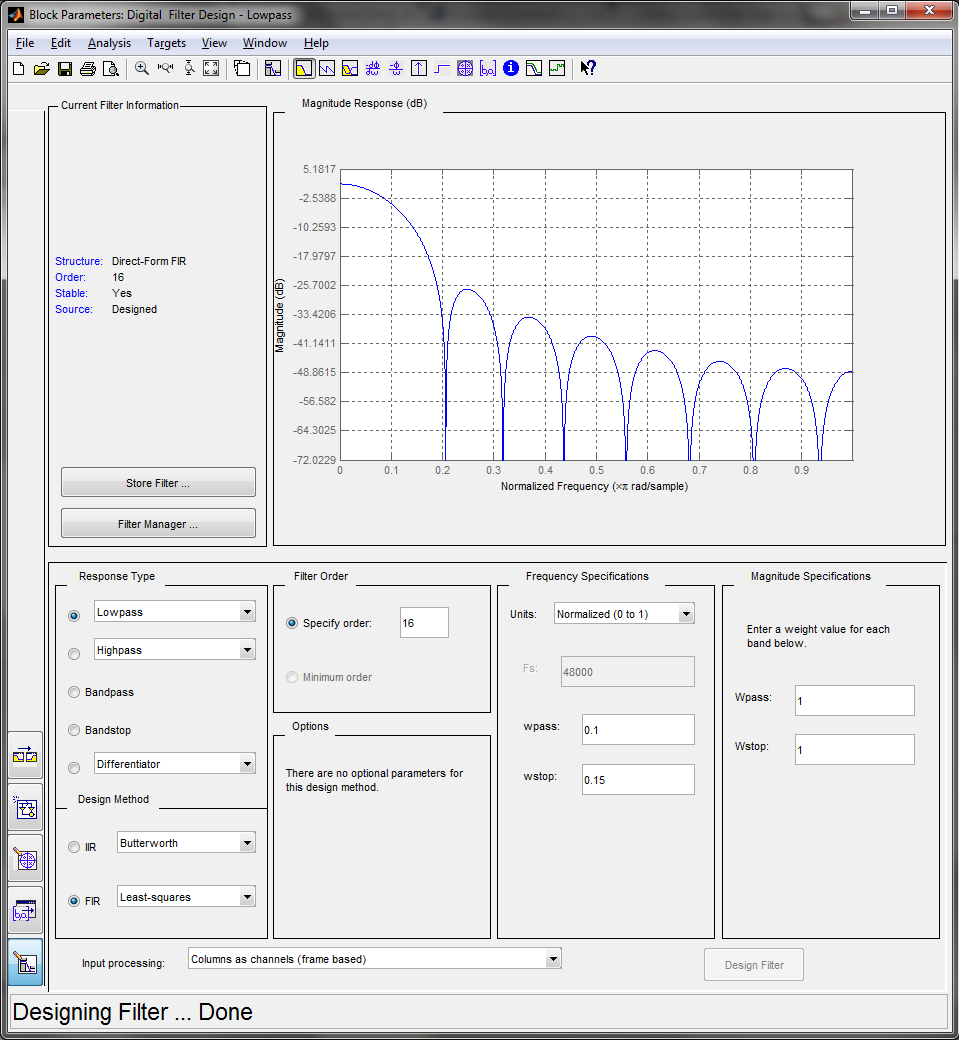
\includegraphics[width=\textwidth]{common/img/filter.png}
                 \vspace{.1cm}
                 \caption{Erstes Filter mit den Parametern wpass~=~0.1 und wstop~=~0.15. Das Ergebnis ist ein schmalbandigeres Filter. }
                 \label{fig:Filter1_A}\textit{}
         \end{subfigure}
%         
\qquad
         \begin{subfigure}[t]{0.5\textwidth}
                 \centering
                 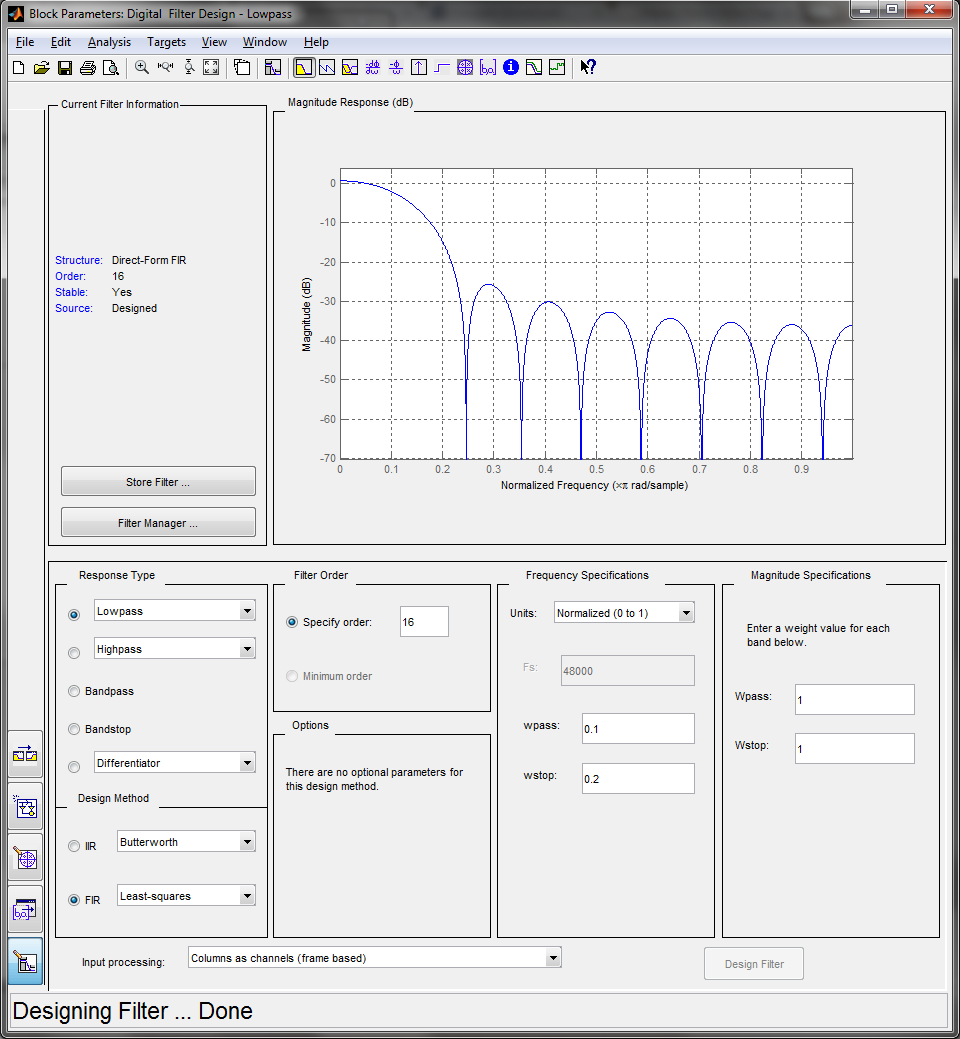
\includegraphics[width=\textwidth]{common/img/filter2.png}
                 \vspace{.1cm}
                 \caption{ Zweites Filter mit den Parametern wpass~=~0.1 und wstop~=~0.2. Der Durchlas bereich ist etwas breiter, dafür sind die Sidelobes stärker gedämpft }
                 \label{fig:Filter2_B}
         \end{subfigure}
%
\end{figure}
%---------------------------------------------------------------------------------------
%\end{landscape}
%
%----------------------------------------------------------------------------
%----------------------------------------------------------------------------
%\newpage
%\begin{landscape}
%	\section{Projektlaufplan KW 31}
%	\label{sec:projectplan}
%	\scalebox{.75}{
%		\begin{ganttchart}[vgrid={draw=none,*1{gray, dashed}},
				hgrid=true,
				today=24,
				title height=1,
				y unit title=0.6cm,
				y unit chart=0.8cm,
				group right shift=0,
				group top shift=.3,
				group height=.3,
				milestone width=.8,
				group peaks={}{}{.2},
				incomplete/.style={fill=black!15}, %
				bar/.style={fill=white}, %
				today label={Heute},
				today rule/.style={dashed, thick}]{44}


\gantttitle{\textbf{2013}}{44} \\
\gantttitlelist{16,...,37}{2} \\
%-------------------------------------------------------------
\ganttgroup{Projekt Evaluation}{3}{14} \\
\ganttbar[progress=100, progress label font=\small\color{black!75},
	progress label anchor/.style={right=4pt}]{Installation der Umgebungen}{3}{6} \\
	
\ganttbar[progress=100, progress label font=\small\color{black!75},
	progress label anchor/.style={right=4pt},
	bar label font=\normalsize\color{black},
	name=rech]{Recherche}{3}{7} \\
	
\ganttmilestone[name=ms1]{Vorstellung der Ergebnisse}{7} \\
	
\ganttbar[progress=90, progress label font=\small\color{black!75},
	progress label anchor/.style={right=4pt},
	bar label font=\normalsize\color{black},
	name=pflichten]
	{Pflichtenheft}{5}{8} \\
	
\ganttmilestone[name=ms2]{Pflichtenheft fertig}{8} \\

\ganttbar[progress=100, progress label font=\small\color{black!75},
	progress label anchor/.style={right=4pt},
	bar label font=\normalsize\color{black},
	name=bNumVerf]
	{Einarbeitung num. Verfahren}{5}{16} \\

\ganttbar[progress=95, progress label font=\small\color{black!75},
	progress label anchor/.style={right=34pt},
	bar label font=\normalsize\color{black},
	name=bCMAES]
	{speziell CMA-ES}{7}{10} \\

\ganttmilestone[name=ms3]{Beurteilung num. Verfahren}{16} \\

\ganttlinkedbar[progress=100, progress label font=\small\color{black!75},
	progress label anchor/.style={right=34pt},
	bar label font=\normalsize\color{black}]
	{Shark Einarbeitung}{17}{18} \\

\ganttlinkedmilestone[name=ms7]{Abschluss Evaluation}{18} \\
	
%-------------------------------------------------------------
\ganttgroup{Erstellung Prototyp}{15}{26} \\
\ganttgroup{(optional)}{15}{18} \\
\ganttbar[progress=25, progress label font=\small\color{black!75},
	progress label anchor/.style={right=4pt},
	bar label font=\normalsize\color{black}]
	{(Entwurf digi. Filter)}{15}{15} \\

\ganttlinkedbar[progress=10, progress label font=\small\color{black!75},
	progress label anchor/.style={right=4pt},
	bar label font=\normalsize\color{black},
	name=bImpFPGA]
	{(Implementation FPGA)}{16}{18} \\

\ganttmilestone[name=ms4]{(Verifikation dig. Filter)}{18} \\
	
\ganttbar[progress=90, progress label font=\small\color{black!75},
	progress label anchor/.style={right=4pt},
	bar label font=\normalsize\color{black},
	name=bImplAlgo]
	{Implementation Algorithmus}{15}{26} \\

\ganttlinkedmilestone[name=ms5]{Implementation Done}{26} \\

%-------------------------------------------------------------
\ganttgroup{Verifikation}{27}{34} \\
\ganttbar[progress=10, progress label font=\small\color{black!75},
	progress label anchor/.style={right=4pt},
	bar label font=\normalsize\color{black},
	name=bVerf]
	{Durchf\"uhrung Verifikation}{27}{34} \\

\ganttlinkedmilestone[name=ms6]{Verifikation Done}{34} \\

%-------------------------------------------------------------
\ganttgroup{Projektdokumentation}{35}{42} \\

\ganttbar[progress=0, progress label font=\small\color{black!75},
	progress label anchor/.style={right=4pt},
	bar label font=\normalsize\color{black},
	name=thesis]
	{Thesis schreiben}{35}{42} \\
	
\ganttmilestone[name=msthesis,milestone label font=\color{red}, 
	milestone/.style={fill=red}]{Abgabe}{42}

%\ganttlink{ms7}{bImplAlgo}
\ganttlink{bImpFPGA}{ms4}
\ganttlink{bNumVerf}{ms3}
\ganttlink{bCMAES}{ms3}
\ganttlink{rech}{ms1}
\ganttlink{pflichten}{ms2}
\ganttlink{thesis}{msthesis}

	\end{ganttchart}
%		}
%\end{landscape}
%
%----------------------------------------------------------------------------

\end{appendix}


\newpage
%- Bibliography --------------------------------------------------------------
\bibliographystyle{ieeetr}
\bibliography{bib/mathesis_collection1}

\end{document}